\documentclass[12pt, a4paper]{article}

% ── Packages ──────────────────────────────────────────────
\usepackage[table]{xcolor}
\usepackage[top=2.5cm, bottom=2.5cm, left=3cm, right=3cm]{geometry}
\usepackage{setspace}
\usepackage{titlesec}
\usepackage{parskip}
\usepackage[T1]{fontenc}
\usepackage[utf8]{inputenc}
\usepackage{mathpazo}
\usepackage{enumitem}
\usepackage{graphicx}
\usepackage{float}
\usepackage{caption}
\usepackage{hyperref}

% ── Prevent orphan/widow lines ────────────────────────────
\widowpenalty=10000
\clubpenalty=10000

% ── Section Formatting ────────────────────────────────────
\titleformat{\section}
  {\Large\bfseries}{\thesection.}{0.8em}{}[\titlerule]

\titlespacing{\section}{0pt}{1.5em}{0.8em}

% ── Caption style ─────────────────────────────────────────
\captionsetup{font=small, labelfont=bf, justification=centering}

% ── Hyperlink style ───────────────────────────────────────
\hypersetup{colorlinks=false}

% ─────────────────────────────────────────────────────────
\begin{document}

% ── Title Page ────────────────────────────────────────────
\begin{titlepage}
  \centering
  \vspace*{3cm}

  {\Huge\bfseries Linux}

  \vspace{1.8cm}

% Students
  {\large\textbf{Student Names:}}\\[0.6em]
  Eslam Yasser Abd Elnaby\\ [0.3em]
  
  Ziad Mohammed Daif\\[0.3em]
  
  Hazem Gamal Abo Zaid

  \vspace{1.8cm}

% Professors
  {\large\textbf{Instructors:}}\\[0.6em]
  Dr.\ Ibtisam Adel \& Dr.\ Amr Abo Hany

  \vfill

  {\large April, 2026}
\end{titlepage}
% Abstract 
\begin{abstract}
This report explores the concept and origins of open-source software and highlights Linux as one of its most important applications. The book addresses the historical roots of the regime and the fundamental contributions of its founders. Furthermore, the report explains why mastering Linux is essential for software and computer science students, focusing on its role as an ideal development environment. Finally, it provides an overview of popular Linux distributions and details of the basic command-line tools needed for efficient system navigation and professional use. 
\end{abstract}

\vspace{3cm}

%index
\tableofcontents
\newpage
% ── Introduction ──────────────────────────────────────────
\setstretch{1.5}

% Section Intro
\section{Introduction}

%figure of Stallman
\begin{figure}[H]
  \centering
  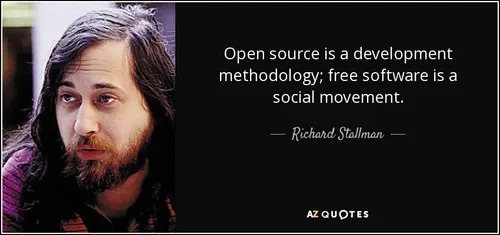
\includegraphics[width=0.65\textwidth]{images/stallman.png}
  \caption{Richard Stallman — founder of the GNU Project and the free software movement}
\end{figure}

In the early 1980s, specifically at the Massachusetts Institute of Technology (MIT), 
The story began. The godfather of the free software movement, Richard Stallman, 
was stallman when he worked in the university's artificial intelligence laboratory. One day, a modern printer 
arrived at the laboratory, and when it encountered some problems, Stallman wanted to 
modify its code (Source Code) to send a notification when the paper broke down, as 
was usual with older devices. But he was surprised that the manufacturer completely 
closed the source under the pretext of copyright and prevented any modification to it. 

This position was the spark of anger that sparked a revolution; Stallman decided that 
monopolizing code was a restriction on programmers' freedom and an obstacle to 
scientific development. Hence, the GNU Project (GNU) was launched in 1983, with 
The aim of building a completely free and open-source operating system, and invited 
Programmers around the world participated in it. 

The project succeeded in building most of the system's core tools and software, but 
The biggest problem remained an obstacle for them: the system's ``core'' (Kernel) was 
incomplete and slow to develop, which disrupted the launch of the entire system. 

%figure linus 
\begin{figure}[H]
  \centering
  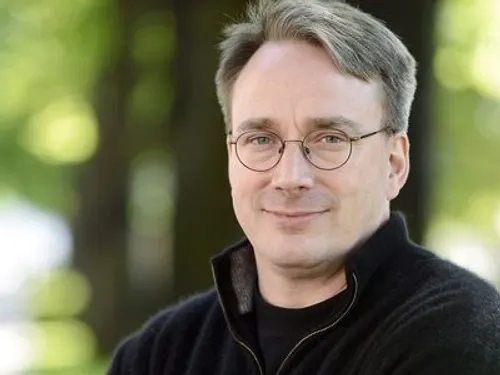
\includegraphics[width=0.5\textwidth]{images/linus.png}
  \caption{Linus Torvalds — creator of the Linux kernel (1991)}
\end{figure}

At about the same time, specifically in 1991, far away in Finland, there was a
university student named Linus Torvalds. Driven by passion and learning, Linus began
writing his own kernel of the operating system from scratch. Without knowing what was going
on at MIT, Linus posted a historical message on a programmer's forum saying that he
was working on a free operating system as a mere ``hobby'', and that it would not be a
huge project.

What happened next changed the shape of technology forever, as the efforts of the
GNU community (which had all the tools of the system but lacked the kernel) met
with the genius of Linus (which had the organized kernel but lacked the tools). The
Two merged to generate the system (GNU/Linux). Thanks to this open
beginning, thousands of programmers around the world turned to develop and modify
the system, and hundreds of distributions (Distributions) branched out from it, sharing
the same powerful kernel and differing in their interfaces and uses, forming the
extended The Linux world that we know today.


\newpage


% Section why do U chosse Linux
\section{Why Linux?}

Many programmers, especially beginners, may ask why professionals use Linux.
We are here to answer this question.

First, Linux is an open-source system that was built through the participation and
contribution of many programmers in 1991, the most famous of whom is Linus, who
built the first kernel model for the system, after which the system was named Linux.
He then made major updates until the system was able to work normally on devices
in September 1991.

Because it is an open-source system, many companies and groups of programmers have
developed it to have hundreds of Linux distributions.

Because of the strength of this system, it has become one of the most important
distributions, and Ubuntu is the leading system in data center servers.

This also encouraged modern languages, like Rust and Go, built for Linux environments. 

\subsection{Reasons why professional programmers use Linux:}

%Important points
\begin{enumerate}[leftmargin=2em, itemsep=0.3em]
  \item The strong organization of the system
  \item It is open source so that you can change anything in the system
  \item Its source code can be modified
  \item It considers the user's privacy
  \item It is light in device resource consumption
  \item Increases productivity
  \item The Terminal and the system are compatible
\end{enumerate}


\newpage


% Section Kernel
\section{Linux Architecture}
The kernel is the most important piece in any system, and Linux is distinguished primarily by the fact that its importance lies in its kernel.
The kernel is the link between the system and the hardware components, without which the hardware components cannot work
as you see in Figure \ref{arch}, \ref{kernal2}, and \ref{kernal1}  to illustrate what the kernel looks like inside the system

\begin{figure}[H]
  \centering
  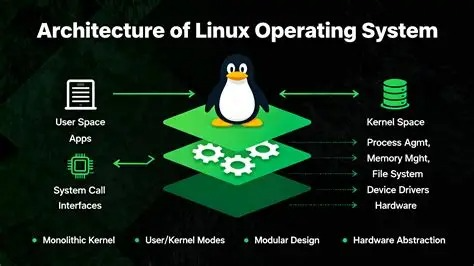
\includegraphics[width=0.5\textwidth]{images/arch.png}
  \caption{Architecture of the Linux operating system}
  \label{arch}
\end{figure}

\begin{figure}[H]
  \centering
  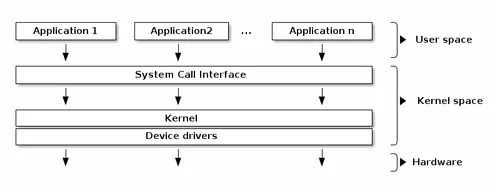
\includegraphics[width=0.5\textwidth]{images/kernal1.png}
  \caption{User Space vs.\ Kernel Space — communication via System Calls}
  \label{kernal1}
\end{figure}

\begin{figure}[H]
  \centering
  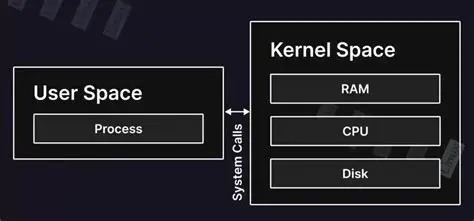
\includegraphics[width=0.5\textwidth]{images/kernal2.png}
  \caption{System Call Interface: the bridge between applications and hardware}
  \label{kernal2}
\end{figure}

\newpage



%Section Distro
\section{Linux Distributions}

Because of the freedom that open-source software provides, over the past two decades, many companies and groups of programmers have created thousands of Linux distributions. Some focus on offering innovative features, while others prioritize absolute stability. Although the Linux ecosystem is extensive, we will highlight only the most popular distributions: 

\subsection{Ubuntu} 
Ubuntu is the most widely used distribution worldwide and has a huge community of enthusiasts. Moreover, its server version is considered one of the best and most reliable in the industry. Ubuntu is easy to use and has strong community support; If you meet any problem, you will find the solution online. It is also worth noting that its solid foundation led to the creation of other phenomenally successful distributions, such as Pop!\_OS and Linux Mint. 

\subsection{Fedora} 
Fedora Powered by popular enterprise software company Red Hat, this distribution is at the forefront of technology. It is often the quickest distro to receive the latest software updates and programming packs, making it a favorite for developers who want the latest tools. 

\subsection{Arch Linux}
Arch Considered one of the most challenging distributions, Arch is primarily aimed at professional programmers and power users. It follows a do-it-yourself philosophy, which means the system comes with barebones. Users must create and customize their systems entirely themselves, including installing the graphical user interface (GUI) and network managers.

There are countless other distributions designed for specific use cases. A quick search for "most popular Linux distributions" will reveal a world of options suitable for every possible need. 

%figure distribution of Linux
\begin{figure}[H]
  \centering
  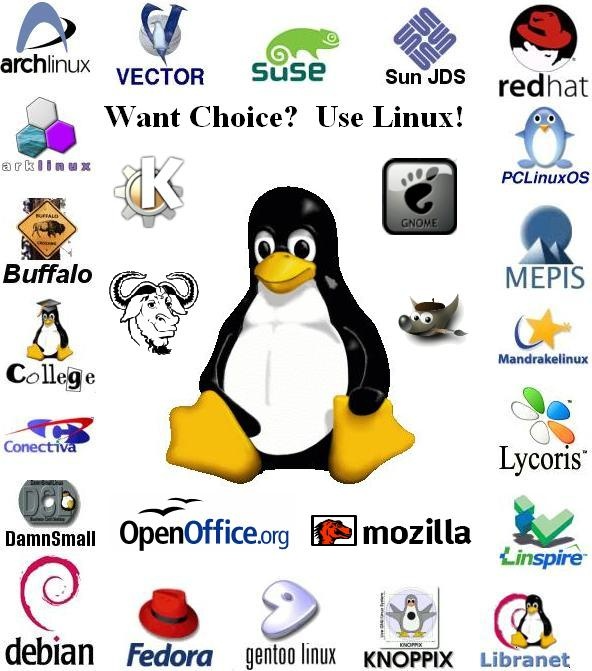
\includegraphics[width=0.5\textwidth]{images/distros.png}
  \caption{A selection of Linux distributions — all sharing the same powerful kernel}
\end{figure}
\newpage




% Section Command Line
\section{Command Line} 
A command line is an instruction that you write on the CLI screen. It is programmed so that each command line does something specific in the system. We will learn about the most famous command lines in This table \ref{commandline}. 

\begin{table}[H] 
    \centering 
    \rowcolors{2}{gray!15}{white}
\begin{tabular}{ l | l | l } 
        \hline 
        \rowcolor{gray!40}
        \textbf{Command} & \textbf{Description} & \textbf{Example} \\ \hline
        
        ls      &	List directory contents.          & ls \\ \hline
        cd      &	Change directory.                 & cd /path/to/directory \\ \hline
        pwd     &	Show current directory.           & pwd \\ \hline
        mkdir   &	Create a new directory.           & mkdir new\_directory \\ \hline
        rmdir   &	Remove an empty directory.        & rmdir empty\_directory \\ \hline
        rm      &   Delete files or directories.      & rm file.txt \\ \hline
        touch   &	Create an empty file.             & touch new\_file.txt \\ \hline
        cp      &	Copy files or directories.        & cp file.txt /path/to/destination \\ \hline
        mv      &	Move or rename files.             & mv file.txt /path/to/new\_location \\ \hline
        cat     &	Display file contents.            & cat file.txt \\ \hline
        nano/vim&   Edit files in terminal.       & nano file.txt \\ \hline
        find    &	Search for files in a directory hierarchy.	& find . -name "file.txt" \\ \hline
        grep    &	Search text using patterns.	      & grep "pattern" file.txt \\ \hline
        tar     &	Archive and compress files.	      & tar -cvf archive.tar file1.txt file2.txt \\ \hline
        df      &	Show disk usage of file systems.  & df \\ \hline
        du      &	Show directory/file size.         & du -sh /path/to/directory \\ \hline
        chmod   &	Change file permissions.          & chmod 755 file.txt \\ \hline
        chown   &	Change file owner.                & chown user:group file.txt \\ \hline
        mount   &	Mount a filesystem.	              & mount /dev/sdb1 /mnt \\ \hline
        umount  &	Unmount a filesystem.             & umount /mnt \\ \hline
    \end{tabular}
    \caption{The most used command line}
    \label{commandline}
\end{table}

\newpage


\section{References}
\begin{enumerate}
    \item Command lines. \url{https://www.digitalocean.com/community/tutorials/linux-commands}
    \item Historical store. \url{https://en.wikipedia.org/wiki/Linus_Torvalds} 
    \item Information about linux. \url{https://kernel.org/category/about.html}
    \item The Linux Kernel documentation. \url{https://kernel.org/doc/html/latest/}
    \item Information about distributions. \url{https://distrowatch.com/}
\end{enumerate}

\end{document}